\section{Section: Prelude}

\section{Section Intro}

\begin{frame}[c]{The Plan}
  \small

  \begin{enumerate}
    \item \textbf{What is cryptography}
    \item \textbf{The end is neigh (quantum attacks)}
    \item \textbf{Migrating to post-quantum cryptography}
    \item \textbf{Advertisement (Migrating your own setup)}
  \end{enumerate}

	\vfill
	\qrcode[height=2.5cm]{https://github.com/rosenpass/slides/blob/main/2025-12-05-howest/slides.pdf}~Slides

  \vfill
\end{frame}



\begin{frame}{Karolin Varner}
  \begin{columns}[fullwidth,c]
	\hspace*{.25\LeftSlideIndent}%
    \begin{column}{\dimexpr.7\linewidth-.25\LeftSlideIndent}
      \begin{itemize}
        \item Initiator \& Lead Scientist off Rosenpass e. V.
        \item Software-Developer \& Cryptographer
        \item Worked for about 12 years in industry with start ups and large corps
        \item Working at Max-Planck-Institute for Security and Privacy since 2024
        \item Worked on Rosenpass \& other cryptographic projects, such as teh X-Wing~cipher
      \end{itemize}
    \end{column}%
    \begin{column}{.3\linewidth}
      \includegraphics[width=.92\linewidth,trim=200 0 100 0,clip]{graphics/karolin-varner.jpg}
    \end{column}
  \end{columns}
\end{frame}

\begin{frame}{Rosenpass e. V.}
  \begin{columns}[fullwidth,c]
  	\hspace*{.25\LeftSlideIndent}
    \begin{column}{.5\linewidth}
      \begin{itemize}
        \item Founded in 2023 as a host for the eponymous project
        \vfill
        \item Security WireGuard VPN against quantum attacks via protocol level hybridization
        \item Institution for translational research in cryptography
        \vfill
        \item Communication hub between science, industry, and civil society
      \end{itemize}
      \bigskip
      \textbf{\url{rosenpass.eu}}
    \end{column}%
    \begin{column}{.5\linewidth}
%      \includegraphics[ width=.92\linewidth]{graphics/Illu-install.png}
		\makebox[\linewidth][c]{\includegraphics[width=1.3\linewidth,page=18]{hpke-slide-designs}\hskip1.5em}
    \end{column}%
  \end{columns}
\end{frame}
